\chapter{Methodology}

\section{Introduction}
The focus of this project is to explore the uses of Naive Bayes in chess and whether it is a viable alternative to current techniques. This chapter will mention the methodology that was used to implement the Naive Bayes classifier in the chess engine. For this project, the python-chess library was highly relied upon. Many different python scripts were used during the project. The main scripts included were \texttt{data\_prep.py} where the data was preprocessed, \texttt{training.py} where the model was trained and evaluated, \texttt{features.py} where the features were calculated, \texttt{game.py} where the game was played and the most important ones \texttt{minimax\_NB\_XXX.py} where the Naive Bayes Classifier was applied to the minimax algorithm.

\section{Random Chess Engine}

\section{Integration of Naive Bayes with Minimax}

\subsection{Data Preparation}

The dataset used for this project was obtained from Kaggle \cite{ChessGameDataset}. The dataset contained over 6.2 million chess games that were played on lichess.com in July 2016. The dataset was in CSV format, making it easy to extract information and analyse. The dataset contained many features, however the only features relevant to this project was the result of the game and the sequence of moves in Algebraic Notation form.

This project wants to explore the how the classification of chess positions into wins and loses can be used to improve the minimax algorithm. For this reason, all games which resulted in a draw were not considered as well as games where one of the players resigned The data was split into 3 different groups to explore how player expetise affects the model's learning and generalisation ability. The first group, named \texttt{master}, was all games where one of the players had an Elo rating of 2200 and above as defined by the Federation International des Echecs (FIDE). The second group, named \texttt{beginner}, were games were both players had an Elo lower than 2200. The last group, named \texttt{random} were games where players with any Elo were considered. The dataset only had 300,000 instances of master games, therefore only 300,000 instances of beginner and random games were used. This is to ensure that the experiments are fair when comparing the effect of group on the model's performance. 

The moves in Algebraic Notation would not provide the Naive Bayes classifier with enough information to classify as it would not provide context of the board state. For this reason, the python-chess library was used to simulate the games. The moves would be extracted from the csv file, then each move would be played on the board. The csv file would be read by using the pandas library and every 6 moves, the features of the board would be extracted and stored, this was to reduce the amount of data to train on as consecutive moves are highly correlated so would not provide more insight for the model. However, end game moves have a bigger affect on the result of the game so in this phase, every other move was used. The last move was also included since this is the move and game state that determined the result of the game. This was also when the results of the games were converted from \texttt{1-0} or \texttt{0-1} to a binary classification where 1 represented a win and 0 represented a loss. This was done to make the model easier to train and evaluate.

\subsection{Feature Selection}

Feature selection is a crucial part of how well the Naive Bayes will perform and generalise. Limited use of features can lead to underfitting and too many features can lead to overfitting. This project also wants to explore the impact different features can have on the model's performance. There were 4 feature sets used in this project. 

The first feature set, considered 4 features: material balance, piece mobility, king attack balance and positional value. Material balance is a very simple feature that considers the difference in number of pieces between the two players, where a positive value indicates a piece advantage for white and a negative value indicates a piece advantage for black. However, each piece is not of equal value in the game, for example a queen has much more power than 2 pawns have. For this reason, the values in Table~\ref{tab:piece_values} were used \cite{shannonXXIIProgrammingComputer1950}. 


\begin{table}[h]
    \centering
    \begin{tabular}{|c|c|}
        \hline
        \textbf{Piece} & \textbf{Value} \\
        \hline
        Pawn & 100 \\
        Knight & 300 \\
        Bishop & 300 \\
        Rook & 500 \\
        Queen & 900 \\
        King & 0 \\
        \hline
    \end{tabular}
    \caption{Values of Chess Pieces}
    \label{tab:piece_values}
\end{table}

Piece mobility is the difference in number of legal moves between the two players. The more moves available to a player suggests that they have more control over the board which could give them a tactical advantage. King attack balance is the difference in number of pieces attacking the king. Most of these features are simple and don't consider the game state as whole, like the position of pieces on the board. Positional value was a feature used where the location of a particular piece on the board can affect how effective it is. An  example of a positional value table for a knight is shown in Table~\ref{tab:knight_positional_values}.

\begin{table}[h]
    \centering
    \begin{tabular}{|c|c|c|c|c|c|c|c|c|}
        \hline
        \textbf{} & \textbf{A} & \textbf{B} & \textbf{C} & \textbf{D} & \textbf{E} & \textbf{F} & \textbf{G} & \textbf{H} \\
        \hline
        \textbf{8} & -50 & -40 & -30 & -30 & -30 & -30 & -40 & -50 \\
        \textbf{7} & -40 & -20 & 0 & 5 & 5 & 0 & -20 & -40 \\
        \textbf{6} & -30 & 0 & 10 & 15 & 15 & 10 & 0 & -30 \\
        \textbf{5} & -30 & 5 & 15 & 20 & 20 & 15 & 5 & -30 \\
        \textbf{4} & -30 & 0 & 15 & 20 & 20 & 15 & 0 & -30 \\
        \textbf{3} & -30 & 5 & 10 & 15 & 15 & 10 & 5 & -30 \\
        \textbf{2} & -40 & -20 & 0 & 5 & 5 & 0 & -20 & -40 \\
        \textbf{1} & -50 & -40 & -30 & -30 & -30 & -30 & -40 & -50 \\
        \hline
    \end{tabular}
    \caption{Positional Value Table for Knight}
    \label{tab:knight_positional_values}
\end{table}

This table favours the knight to be in the centre of the board rather than the edge. This is because when the knight is is in the centre, it can control more squares so has more opportunity to attack and defend, whereas when it is near the edge, the knight is more restricted, especially the corners where it only has 2 possible moves.

The second feature set considered the same features as the first set but also included the control of the centre. This is defined by the number of pieces within the centre. Again, it calculates the difference between the white and black pieces in the middle. This feature was implemented as two separate features, one for the 2x2 square in the middle and one for the 4x4 square in the middle as shown in Figure~\ref{fig:centres}.

\begin{figure}[h]
    \centering
    \begin{subfigure}[t]{0.4\textwidth}
        \centering
        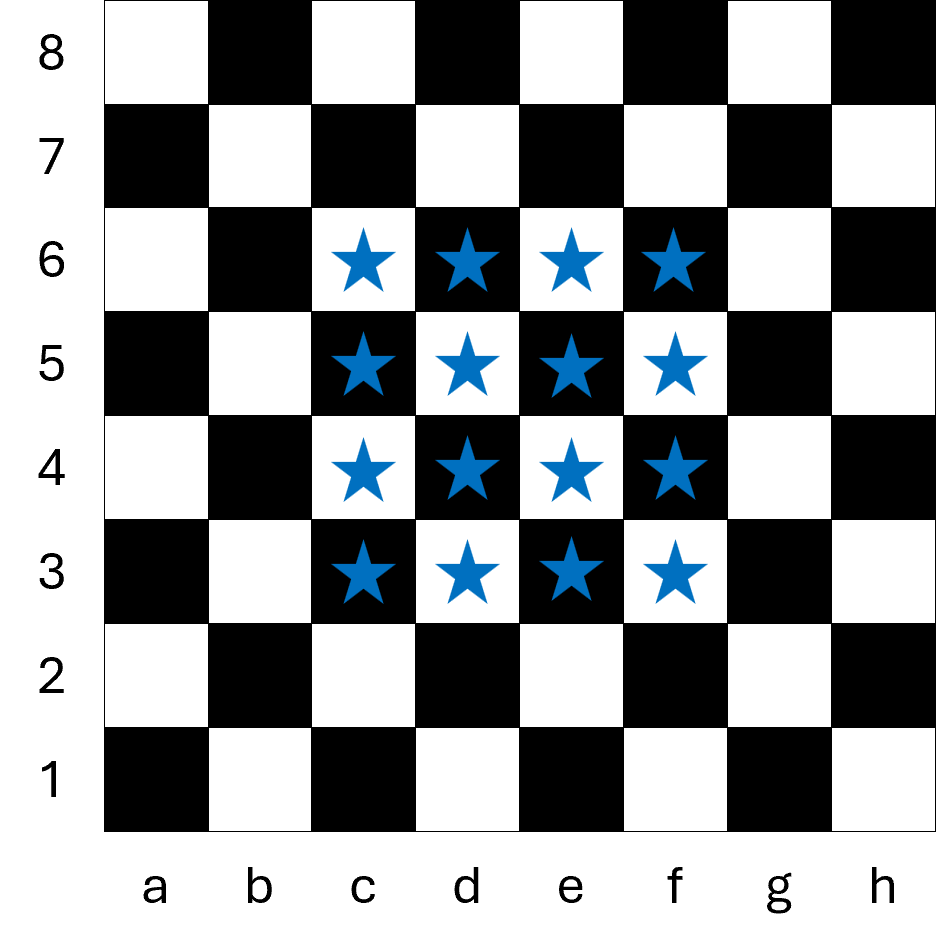
\includegraphics[width=\textwidth]{images/bigCentre.png}
        \caption{Big centre of the Board}
        \label{fig:bigcentre}
    \end{subfigure}
    \hfill
    \begin{subfigure}[t]{0.4\textwidth}
        \centering
        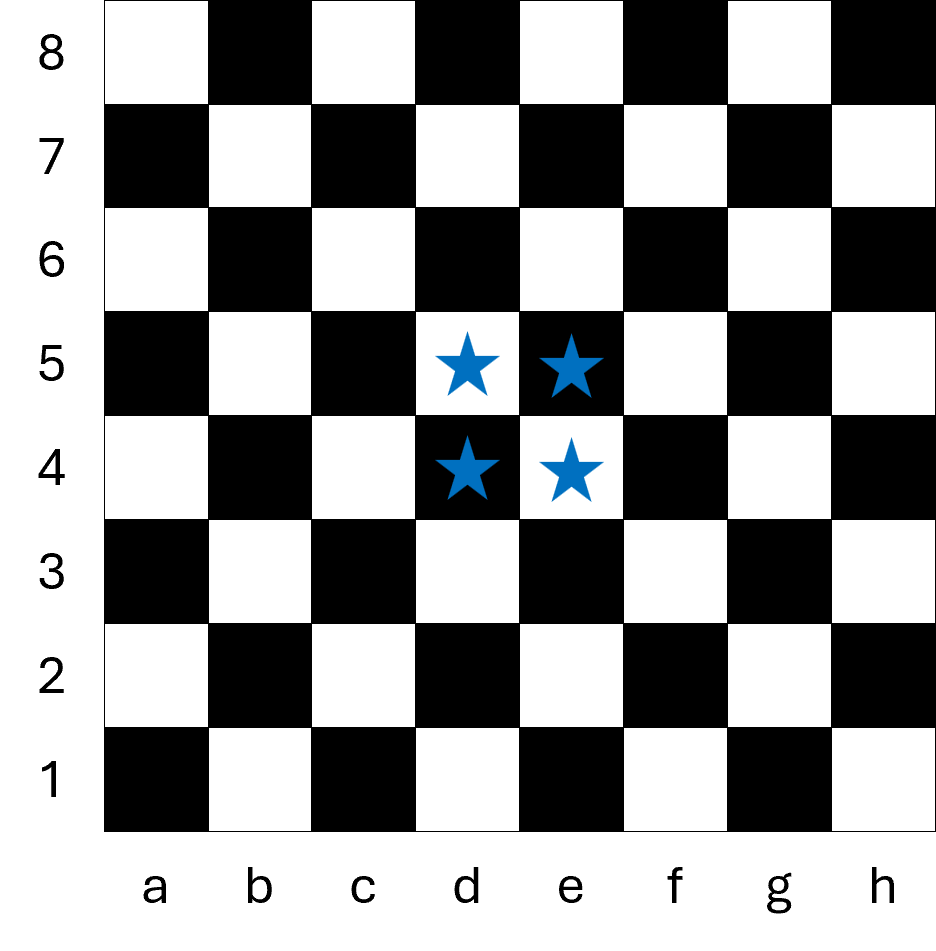
\includegraphics[width=\textwidth]{images/smallCentre.png}
        \caption{Small centre of the Board}
        \label{fig:smallcentre}
    \end{subfigure}
    \caption{Comparison of the small and big centres of the board.}
    \label{fig:centres}
\end{figure}

The third feature set explored in this research considers all of the features mentioned previously but also more complex features, specifically pawn structure. The structure of pawns can determine how much control the player has, defending its pieces and preventing advancements from the enemy. Two structures were used for this project, isolated pawns and doubled pawns. Isolated pawns are pawns that do not have any friendly pawns on adjacent files. Usually this is considered as a weak structure since they can't be defended by other pawns and also can be easily blocked by the opponent pieces. However, some times it could be a powerful structure as it can have more control over the board and also some openings use isolated pawns in order to allow more movement for rooks and bishops. 
% TODO: Reference ann maybe pictures of isolated or doubled pawns
Doubled pawns are pawns that are on the same file. Generally this is a weak structure since they are limiting each other's mobility and can generally become isolated. However creating doubled pawns can be used to open up files or diagonals for rooks and bishops.

The last feature set used included all the features in the third feature set but also more complex features. This included the castling rights of the player, king safety and game phase. Castling is a move that allows the king to move two squares towards a rook. This is a very strong move as it allows the king to move away from the centre where it is generally more dangerous. It also allows the rook to have a more active role in the game. Therefore being able to retain the ability to perform this act can influence the game majorly. For the purpose of this project, the castling rights were considered for both kingside and queenside. King attack balance is a very simple feature which only considers the number of pieces attacking the king.  For this feature set a more complex attribute was used, king safety. King safety calculates the number of pawns in adjacent squares, which is known as pawn shield, and also calculates the number of pieces attacking adjacent squares to the king then returns the difference between the two. The last feature included in this feature set was game phase. This would output one of 3 values, opening, middle game or end game. This was calculated by giving values to each type of piece and summing up all the pieces on the board. Then the percentage of pieces left in the board was calculated. If it was more than 66\% it returned 0 for opening, if it was between 33\% and 66\% it returned 1 for middle game and if it was less than 33\% it returned 2 for end game.

\subsection{Naive Bayes Classifier}

There are many resources available to implement the Naive Bayes Classifier, the most commonly used is the one provided by the scikit-learn library. For this project, having complete control and understanding of the model was important, therefore the Naive Bayes Classifier was implemented from scratch. This allowed for more flexibility in the implementation and allowed for more experimentation with the model. 

The main steps of the Naive Bayes Classifier are as follows:


1. Calculate the prior probabilities of each class.

2. Calculate the likelihood of each feature given the class.

3. Calculate the posterior probability for a class given a set of features using Bayes' theorem.

4. Predict the class of a new instance by choosing the class with the highest posterior probability for that feature.

The prior probabilities were calculated by counting the number of instances in each class then dividing it by the total number of instances. The numpy library was used to make this process more efficient. Then since for this project, continuous attributes were used, the Gaussian implementation of Naive Bayes was used, therefore after calculating the prior probabilities, the mean and standard deviation of each feature was calculated for each class, again aided by the numpy library.  The likelihood was then calculated for each using the Gaussian formula as given in Equation~\ref{eq:gaussianEquation}.


\begin{equation}
    \label{eq:gaussianEquation}
    P(X | C) = \frac{1}{\sqrt{2\pi\sigma^2}} e^{-\frac{(x - \mu)^2}{2\sigma^2}}
\end{equation}

Then these likelihoods were used to calculate the posterior probabilities for each class given the set of features, which is done by using Bayes' theorem. Due to the assumption of conditional independence, the posterior probability can be simplified to the product of the prior probability and the likelihood of each feature given the class. Once the posterior probabilities were calculated, the class with the highest posterior probability was chosen as the predicted class. Two functions were implemented, \texttt{predict} and \texttt{predict\_prob}. \texttt{predict\_prob} returns the posterior probabilities for each class given a set of features which can be used to compare the confidence of the classifiers predictions. The \texttt{predict} function returns the class which the model classified the instance with, ie. the class with the highest posterior probability

Naive Bayes consists of the multiplication of multiple probabilities, which can lead to very small numbers causing underflow issues. To overcome this, the logarithm of the probabilities was used to predict the class. This then caused rise to another issue, the fact that $log(0)$. Due to the nature of the classifier, this could possibly occur. To prevent this from occurring, a small constant was added to the probabilities before taking the logarithm. This constant was set to 0.1. This was a small enough constant to not affect the results of the model but also large enough to prevent underflow issues.

The features that were extracted from the data was then used to train the model. The data was split into 80\% for training and 20\% for testing. This ratio is ideal as it provides enough data allow the model to learn and generalise well while enough to still test it's effectiveness. The features outlined in the previous section can all be in different scales which could give more importance to some features over others. Before feeding the data into the model, the data was standardised by using the StandardScaler from the scikit-learn library.  This ensured that all features were on the same scale so the model would not be biased towards any feature. After training the models they were saved using the joblib library which allowed the use of the model without needing to retraining the model every time. Since there are 3 different groups of data and 4 feature sets, a total of 12 models were trained. 

\subsection {Model Evaluation}

After training the model, it is important to know how well the model performs and how well it generalises to new data. Evaluating models also allows comparison of the findings with other findings in the literature. There are many ways to evaluate a classifier and for this project we will calculate a number of different metrics to gain a holistic view of the model's performance. The first metric calculated was the accuracy of the model. This is the most straightforward measure of the model's overall correctness, by providing the proportion of predictions that were correct \ref{eq:accuracy}.


\begin{equation}
    \label{eq:accuracy}
    \text{Accuracy} = \frac{\text{Correctly Classified Instances}}{\text{Total Instances}}
\end{equation}

Where correctly classified instances is the sum of True Positives and True Negatives. The next two metrics calculated for the model were precision and recall. Precision is the proportion of true positive predictions to the total number of positive predictions made by the model. This is an important metric to consider because it provides insight into how many of the positive predictions made by the model were actually correct. Recall is the proportion of true positive predictions to the total number of actual positive instances in the dataset. This metric is important because it provides insight into how many of the actual positive instances were correctly predicted by the model. The equations for precision and recall are given in Equations~\ref{eq:precision} and \ref{eq:recall} respectively. These two metrics are usually related as there is a trade off between the two, generally increasing one causes the other to decrease.

\begin{equation}
    \label{eq:precision}
    \text{Precision} = \frac{\text{True Positives}}{\text{True Positives} + \text{False Positives}}
\end{equation}


\begin{equation}
    \label{eq:recall}
    \text{Recall} = \frac{\text{True Positives}}{\text{True Positives} + \text{False Negatives}}
\end{equation}


Usually it is more convenient to compare models using a single metric, which takes into account both precision and recall. $F_{\beta}$ score is the weighted harmonic mean of precision and recall, providing a metric that balances the two. The $\beta$ parameter allows control over the trade-off between precision and recall.  A $\beta$ value of 1 gives equal importance to precision and recall which is what will be used for this project. 

\begin{equation}
    \label{eq:f1}
    F_{\beta} = (1 + \beta^2) \cdot \frac{\text{Precision} \cdot \text{Recall}}{\beta^2 \cdot \text{Precision} + \text{Recall}}
\end{equation}

The last metric used is the kappa statistic. This is a measure of how well the model performs compared to a random classifier. The benefit of this metric is that it takes into account the possibility of the model being correct by chance. The equation for the kappa statistic is given in Equation~\ref{eq:kappa} .

\begin{equation}
    \label{eq:kappa}
    \kappa = \frac{p_o - p_e}{1 - p_e}
\end{equation}

Where $p_o$ is the observed accuracy of the model and $p_e$ is the expected accuracy of the model. The expected accuracy is calculated by multiplying the proportion of instances in each class by the proportion of instances in each class. The kappa statistic is commonly understood by the categorisation in Table~\ref{tab:kappa} \cite{landisMeasurementObserverAgreement1977}. 




\begin{table}
    \centering
    \begin{tabular}{|c|c|}
        \hline
        \textbf{Kappa Value} & \textbf{Agreement level} \\
        \hline
        $<$ 0 & Poor agreement \\
        0.01 - 0.20 & Slight agreement \\
        0.21-0.40 & Fair agreement \\
        0.41-0.60 & Moderate agreement \\
        0.61-0.80 & Substantial agreement \\
        0.81-1.00 & Almost perfect agreement \\
        \hline
    \end{tabular}
    \caption{Interpretation of Kappa Statistic}
    \label{tab:kappa}

\end{table}



\subsection{MMNB Algorithm}

The MMNB algorithm is a combination of the Naive Bayes Classifier and the traditional minimax algorithm. There were two implementations used for this project, one where the Naive Bayes completely replaced the evaluation function of the minimax algorithm and one where the Naive Bayes was used to improve the evaluation function by using it in conjunction with a traditional evaluation function. 

The first implementation was built in the \texttt{minimax\_NB\_sub.py}. The benefit of the Naive Bayes classifier over other classifiers is that it can provide how confident the model is in its predictions in the form of probabilities. In this version of MMNB, a standard minimax algorithm with alpha-beta pruning was used. Due to limitations in computational power and time, a depth of 3 was used. This allowed enough exploration of the game tree that it can be an informed decision but also to do this in a reasonable time period. When the maximum depth is reached or it met a terminal node (ie. the game has terminated with a win, lose or draw) then instead of calling a traditional evaluation function, an evaluation function implementing Naive Bayes was used. 

In the revised evaluation function, the model and scaler were loaded from the joblib files. The board state is passed to the features function to extract the current features of the board. The features are then scaled using the loaded scaler. These features are then fed to the predict\_prob function of the Naive Bayes Classifier. This function would then return the posterior probabilities for both classes, win and loss. These probabilities are then used to calculate the value of the node. The value of the node is calculated by taking the difference between $P(Winning | X)$ and $P(Losing | X)$. The value is positive when the classifier thinks white is at an advantage and negative when it thinks black is at an advantage. Terminal nodes also need to be considered, so if the board state is in a checkmate position, the naive bayes evaluation would be disregarded and a value of $\pm \infty$ would be returned dependant on the player who has won. The value of this evaluation function is then returned to the minimax algorithm where it continues to search the rest of the game tree. 

The second implementation took a more traditional approach to the minimax algorithm. The Naive Bayes was not solely used but rather a combination of both was used to make a more informed evaluation score. This was implemented in the \texttt{minimax\_NB\_integrated.py} file. The minimax algorithm was implemented in the same way as the previous implementation, but when the maximum depth was reached or a terminal node was reached, a different version of the evaluation function will be used. In this function two factors were considered. The first was the Naive Bayes score, this was wen through the same process as the previous implementation. The second used was a more traditional evaluation which considered material balance and positional value. The material balance was calculated using the same values as used during the feature extraction for the Naive Bayes model \ref{tab:piece_values}. The positional values were also calculated similar to what was used for the feature extraction \ref{tab:knight_positional_values}. These two values were summed up and used as the traditional score. The traditional score and Naive Bayes score will be at very different scales, which would cause the traditional score to dominate the Naive Bayes score. To prevent this, the traditional score was normalised to be between 0 and 1. This was done by taking the maximum and minimum values of the traditional score and scaling it to be between 0 and 1. Due to the fact that the logarithm of the probabilities were used to calculate the Naive Bayes score, the Naive Bayes score was also scaled to be between 0 and 1. This was done by applying the softmax function to the Naive Bayes score, given by the equation \ref{eq:softmax}. 


\begin{equation}
    \label{eq:softmax}
    \text{softmax}(x_i) = \frac{e^{x_i}}{\sum_{j=1}^{n} e^{x_j}}
\end{equation}


The two scores were then combined by taking the weighted sum of the two scores. The default weights were set to 0.5 for both, however, during experiements it will be explored how the weights affect the performance of the minimax algorithm. The final score is then returned to the minimax algorithm where it continues to search the rest of the game tree.





% \section{Introduction}
% As mentioned previously, the focus of this paper is to explore the uses of Naive Bayes in chess and how this could impact other domains in computer science. This chapter will mention the methodology that was used to implement the Naive Bayes classifier in the chess engine. 

% \section{Random Chess Engine}
% % ??????Initially I wrote code to visualise the chess board. This makes it easier to to understand the game state and see what moves my chess engine would make. This makes it easier to understand my engine as well as debugging issues it may have. ????[SHOULD I INCLUDE THIS]

% For the purpose of this project, the python-chess library will be used as a base to create chess engine. The reason for this choice of library is because it has integrated features needed for this project. This includes support for FEN notation, methods to get legal moves, and also it was also chosen due to the optimisations it uses including representing the board as a bitboard.

% The first step was to create a chess engine engine that randomly picks moves. This implementation was very simple due to python-chess' method \textit{board.legalmoves()} which provides all the legal moves available to the current player. Using this list of moves, one is then chosen at random. The purpose of this random engine is be used as a benchmark for the main chess engine to be created.

% \section{MiniMax and Alpha-Beta pruning}
% Minimax is used by the majority of chess engines. The aim is to implement Naive Bayes to improve the minimax algorithm. So intuitively the first step is implement minimax. Alpha-Beta is much more powerful than basic minimax as it will always give the same output as minimax and is much faster. Therefore, Alpha-Beta will be used directly. This is the pseudocode for the algorithm used. A similar method is use for alphaBetaMin.
% % ????UPDATE pseudocode???
% \begin{algorithm}[h]
%     \caption{Alpha-Beta Pruning Algorithm}
%     \begin{algorithmic}
%         \Function{AlphaBetaMax}{Board, Alpha, Beta, Depth}
%         \If{Depth = 0 or Game Over}
%             \State \Return \Call{Eval}{Board}, None
%         \EndIf
%         \State $BestValue \gets -\infty$
%         \State $BestMove \gets$ None

%         \For{each Move in legal\_moves}
%             \State \Call{MakeMove}{}
%             \State $Score \gets \textsc{AlphaBetaMin}(Board, Alpha, Beta, Depth - 1)[0]$
            
%             \If{Score \textgreater \ BestValue}
%                 \State $BestValue \gets Score$
%                 \State $BestMove \gets Move$
%                 \State $Alpha \gets \max(Alpha, Score)$
%             \EndIf
%             \If{Score \textgreater= Beta}
%                 \State \textbf{break}
%             \EndIf
%         \EndFor
%         \State \Return $BestValue, BestMove$
%         \EndFunction
%     \end{algorithmic}
% \end{algorithm}

% When using alpha-beta pruning, a depth of 3 was used. This was due to the limited computational power available. The depth of the search tree is a primary factor that determines the performance of the chess engine. The higher the depth, the more possibilities the engine can explore which means each move made would have been given more consideration resulting in a better move.

% The other factor of the minimax algorithm that is important is the evaluation function. This is what determines the moves that are made. It gives a value to a game state to approximate which player is winning at that point in time as it is infeasible to search the entire game tree. So the evaluation function is used to estimate the winner at a certain point in the game. The evaluation function used for the purpose of this project will be very simple and will be mainly based on material balance. This is a good indicator of the current state of the game as generally the more pieces a player has the more options they have, therefore they are more likely to win.

% \begin{equation}
%     \label{eq:material_1}
%     \text{Material Balance} = \text{Number of White Pieces} - \text{Number of Black Pieces} 
% \end{equation}


% However, considering each piece of equal value is not representative of the true value of pieces during the game. For example 1 queen is worth more than 2 pawns. Therefore, this research will use the values in Table~\ref{tab:values} to calculate the material balance, which are the commonly accepted values for each piece \cite{guptaDeterminingChessPiece2023}.

% \begin{table}[h]
%     \centering
%     \begin{tabular}{|c|c|}
%         \hline
%         \textbf{Piece} & \textbf{Value} \\
%         \hline
%         Pawn & 100 \\
%         Knight & 300 \\
%         Bishop & 300 \\
%         Rook & 500 \\
%         Queen & 900 \\
%         King & 0 \\
%         \hline
%     \end{tabular}
%     \caption{Values of Chess Pieces}
%     \label{tab:values}
% \end{table}

% This evaluation function is relatively strong and incentivises the engine to take pieces when possible and also to protect its own pieces. After testing this evaluation function, as expected, the engine was winning initially by taking pieces. However, it never won against the random engine. After analysing the games played, the problem was in the end game. The evaluation function did not incentivise the engine to check the opponent, which is the most important part of chess. Therefore, checkmates were considered terminal nodes by giving them a value of $\pm \infty$ dependant on the player that is winning. A value of 10 was also given to check as this is a very strong move. 
% % This was then the ???final??? evaluataion function used.


% \section{Data Collection}

% The choice of dataset used for the Naive Bayes Classifier was an important task to ensure the classifier had enough data to be trained on but also have good data to be trained on. There were many datasets that were considered, however in the end, the dataset from kaggle.com was used 
% % [REFERENCE] 
% which had 6.25 million chess games played on lichess.com in July 2016 . This provided a lot of flexibility as there is a lot of data to train on. There were other datasets like a set of 4 million games on chess.com only played with grandmaster players. However, the aim is to train a model to work for all level of players so the lichess database was chosen. 

% The lichess dataset was in csv format. These are the features that were part of the dataset:

% \begin{itemize}
%     \item \textbf{Event:} The type of game.
%     \item \textbf{White:} White's ID.
%     \item \textbf{Black:} Black's ID.
%     \item \textbf{Result:} The outcome of the game (\texttt{1--0} if White wins, \texttt{0--1} if Black wins and \texttt{1/2--1/2} if they draw).
%     \item \textbf{UTCDate, UTCTime:} The date and time (UTC) when the game was played.
%     \item \textbf{WhiteElo, BlackElo:} ELO of the players.
%     \item \textbf{WhiteRatingDiff, BlackRatingDiff:} The change in rating points after the game.
%     \item \textbf{ECO:} Opening in ECO (Encyclopaedia of Chess Openings) encoding,
%     \item \textbf{Opening:} Opening name.
%     \item \textbf{TimeControl:} The time allocated for each player, plus any increment in seconds.
%     \item \textbf{Termination:} The reason the game concluded.
%     \item \textbf{AN (Algebraic Notation):} The sequence of moves in algebraic notation.
% \end{itemize}

% A lot of the features would not be very useful to train the model. The ID's of the players would not be useful to train with so was discarded. The UTCDate, UTCTime also would not be useful as the time of day a game is played wouldn't affect the outcome of the game or to decide the best move to make. The Elo ratings of the players would be useful as players of similar levels may play in similar ways however this also wasn't used as this information won't always be available when using the engine. The way the game terminated is also information that wouldn't be beneficial as all that is important is the final game result. The most important features that was utilised was the result of the game and the sequence of moves in algebraic notation.

% The data then needed to be preprocessed. The moves in algebraic notation needed to be converted in a format that can be used by the Naive Bayes Classifier. For each game, the python-chess library to simulate the game, so for each move the board is updated. However using every move would be too much data to train on, especially since consecutive moves are highly correlated. Therefore, for most of the game the features at every 6 moves was used however during end game, every other move was used. This is because during the end game, each move will most likely have a bigger impact on the result of the game. For the purpose of this project, end game is after 75\% of the moves have been made. The last move is also included in the data as this is the move that determined the result of the game.
% \section{Feature Selection}

% Material balance is the first feature implemented. Arguably this is the most important feature to estimate the current state of a chess game. For the purpose of this project, the values in Table~\ref{tab:values} were used to calculate the material balance, using Equation~\ref{eq:material_2}. The material balance is positive if the values of White's pieces are grater than the values of Black's pieces and vice versa.
% \begin{equation}
%     \label{eq:material_2}
%     \text{Material Balance} = \text{Number of White Pieces} - \text{Number of Black Pieces} 
% \end{equation}

% Another feature used is the positional value of pieces. The location of specific pieces on the board can influence how effective it is within the game. An example of a piece position table is given in Table~\ref{tab:knight_positional_values} to calculate the positional value of a knight.

% \begin{table}[h]
%     \centering
%     \begin{tabular}{|c|c|c|c|c|c|c|c|c|}
%         \hline
%         \textbf{} & \textbf{A} & \textbf{B} & \textbf{C} & \textbf{D} & \textbf{E} & \textbf{F} & \textbf{G} & \textbf{H} \\
%         \hline
%         \textbf{8} & -50 & -40 & -30 & -30 & -30 & -30 & -40 & -50 \\
%         \textbf{7} & -40 & -20 & 0 & 5 & 5 & 0 & -20 & -40 \\
%         \textbf{6} & -30 & 0 & 10 & 15 & 15 & 10 & 0 & -30 \\
%         \textbf{5} & -30 & 5 & 15 & 20 & 20 & 15 & 5 & -30 \\
%         \textbf{4} & -30 & 0 & 15 & 20 & 20 & 15 & 0 & -30 \\
%         \textbf{3} & -30 & 5 & 10 & 15 & 15 & 10 & 5 & -30 \\
%         \textbf{2} & -40 & -20 & 0 & 5 & 5 & 0 & -20 & -40 \\
%         \textbf{1} & -50 & -40 & -30 & -30 & -30 & -30 & -40 & -50 \\
%         \hline
%     \end{tabular}
%     \caption{Positional Value Table for Knight}
%     \label{tab:knight_positional_values}
% \end{table}

% This table favours the knight to be in the centre of the board rather than the edge. This is because when the knight is in the centre it can control more squares and has more options whereas when it is near the edge, the knight is much more restricted, especially the corners where they have only 2 possible moves. Another example are pawns which are also more valuable in the centre of the board but also in squares that are close to promotion. They are usually not effective in the starting ranks. The positional values of all the black pieces are then summed up and subtracted from the sum of the positional values of the white pieces.

% Another feature considered for the Naive Bayes Classifier is piece mobility. Piece mobility is the possible moves a piece can make. Generally the more moves available to a player, the more control they can have over the board. This is calculated as the difference between the number of legal moves White has and the number of legal moves Black has.

% King Safety is another feature that is critical to the game. The winning or losing of the game solely lies upon how well you cant protect the king. There are many ways to define king safety. In this project, we will use the amount of pieces that are attacking the king. This is an important factor to consider since, the more pieces attacking the king, the more likely the player is to lose.

% Structure of pawns was also considered as a feature. The structure of pawns can determine how much control the player has, defending its pieces and preventing advancements from the enemy. The two that were considered was isolated pawns and doubled pawns. Isolated pawns are pawns that do not have any friendly pawns on adjacent files. Usually this is a weak structure since they can't be defended by other pawns and also can be easily blocked by the opponent pieces however they can be considered strong in some cases. This is because they can have more control over the board but also some openings use isolated pawns in order to allow more movement for rooks and bishops. Doubled pawns are pawns that are on the same file. Generally this is a weak structure since they are limiting each other's mobility and can generally become isolated. However creating doubled pawns can be used to open up files or diagonals for rooks and bishops.

% The last feature considered is the castling rights of the player. Castling is a move that allows the king to move two squares towards a rook. This is a very strong move as it allows the king to move away from the centre which is generally more dangerous. It also allows the rook to have a more active role in the game. Whether the play has castling rights both kingside and queenside are considered. 

% After collecting all the features, I standardised the data. This is because the features are on different scales so it's important to normalise the data to ensure the Naive Bayes Classifier is trained properly and doesn't give importance to features that are on a larger scale. I utilised the StandardScaler from the scikit-learn library. This is done by the following formula:

% \begin{equation}
%     \label{eq:standardisation}
%     z = \frac{x - \mu}{\sigma}
% \end{equation}

% \begin{itemize}
%     \item $x$: Feature value
%     \item $\mu$: Mean of the feature
%     \item $\sigma$: Standard deviation of the feature
% \end{itemize}

% This allows all the features to have a mean of 0 and a standard deviation of 1 but also keep the original distribution of the data.


% \section{Naive Bayes Classifier}

% The Naive Bayes Classifier is a simple classifier that is based on Bayes' Theorem. Bayes' theorem is a fundemental principle that describes how the new evidence can change the probability of an event. Bayes' Theorem is given by the following equation:

% \begin{equation}
%     \label{eq:bayes}
%     P(A|B) = \frac{P(B|A) \cdot P(A)}{P(B)}
% \end{equation}

% Where:
% \begin{itemize}
%     \item $P(A|B)$: Posterior probability
%     \item $P(B|A)$: Likelihood
%     \item $P(A)$: Prior probability
%     \item $P(B)$: Evidence probability 
% \end{itemize}

% Posterior probabilty is the probability of event A happening after knowing new evidence B. Likelihood is the probability of evidence B happening given that event A is true. Prior probability is the probabilty of event we intiially know about A before any new evidence. 

% The first step for implementing Naive Bayes is to calculate the prior probabilities of each class. This is calculated by going through the whole dataset and working out the proportion of each class. This is done by the following formula:

% \begin{equation}
%     \label{eq:prior}
%     P(C) = \frac{N_c}{N}
% \end{equation}

% Where:
% \begin{itemize}
%     \item $P(C)$: Prior probability of class C
%     \item $N_c$: Number of instances of class C
%     \item $N$: Total number of instances
% \end{itemize}

% The next step is to calculate the likelihood of each feature given the class. Ther are two main type of Naive Bayes classifiers, Gaussian and Multinomial. Multinomial is used for discrete features, calcluating the likelihood based on the count of each feature. 

% \begin{equation}
%     \label{eq:multinomial}
%     P(X | C) = \frac{N_{X,C} + 1}{N_C + V}
% \end{equation}

% Where:
% \begin{itemize}
%     \item $N_{X,C}$: Number of instances of the feature $X$ in class $C$
%     \item $1$: Laplace smoothing constant
%     \item $N_C$: Number of instances in class $C$
%     \item $V$: Number of possible values for $X$
% \end{itemize}

% However, most of the features used in this project are continuous so Guassian Naive Bayes is more ideal. Gaussian Naive Bayes calculates the likelihood, assuming the features are normally distributed. This is done by the following formula:

% \begin{equation}
%     \label{eq:gaussian}
%     P(X | C) = \frac{1}{\sqrt{2\pi\sigma^2}} e^{-\frac{(x - \mu)^2}{2\sigma^2}}
% \end{equation}

% Where:
% \begin{itemize}
%     \item $x$: Feature value
%     \item $\sigma$: Standard deviation of the feature
%     \item $\mu$: Mean of the feature
% \end{itemize}

% Then we need to work out the Posterior probability for a class given a set of features $X = x_1, x_2, ..., x_n$ by using Bayes' theorem. Naive Bayes assumes that the features are conditionally independent given the class, which allows us to simplify the equation as the product of the likelihoods. This is done by the following formula:

% \begin{equation}
%     \label{eq:posterior}
%     P(c | X) = \frac {P(c) \prod_{i=1}^{n} P(x_i | c)} {P(X)}
% \end{equation}

% Where:
% \begin{itemize}
%     \item $P(c | X)$: Posterior probability of class $c$ given features $X$
%     \item $P(c)$: Prior probability of class $c$
%     \item $P(x_i | c)$: Likelihood of feature $x_i$ given class $c$
%     \item $P(X)$: Evidence probability
% \end{itemize}

% Then this is used to predict the class of a new instance by choosing the class with the highest posterior probability for that feature. Since $P(X)$ is the same for each class, it can be removed when comparing the posterior probabilities. 

% \begin{equation}
%     \label{eq:posterior}
%     P(c | X) \propto P(c) \prod_{i=1}^{n} P(x_i | c)
% \end{equation}

% So then the predicted class of an instance is chosen by the following formula:

% \begin{equation}
%     \label{eq:prediction}
%     \hat{y} = \arg\max_{c} P(c) \prod_{i=1}^{n} P(x_i | c)
% \end{equation}

% When doing calculations, since we are working with probabilities which are small numbers and multiplying them can result in very small numbers, causing underflow problems. To prevent this, we can use the log of the probabilities which also converts the multiplications to additions, given by this formula:

% \begin{equation}
%     \label{eq:log}
%     \log(P(c | X)) \propto \log(P(c)) + \sum_{i=1}^{n} \log(P(x_i | c))
% \end{equation}

% A small constant $\epsilon$ is added to the likelihoods to prevent taking the logarithm of 0.


% \section{Model Training}

% The Naive Bayes Classifier was then train on the preprocessed data. Due to restrictions on available computing power, only a small subset of the data was used to train the model. The data was split into a training set and testing set, where 80\% was used for training and 20\% was used to test the model. This is usually the standard way to split data to train the model with the majority of the data but also test it on data it hasn't seen before to see how well it generalises.

% \section{Model Evaluation}

% % ??? Maybe include Kappa score????

% After training the model, we are interested in knowing how well the model performs and generalises to new data. There are many ways to evalutate a model. One way to do this is to use a confusion matrix. A confusion matrix is a table that shows how well the model classfied instances. The confusion matrix is shown in Table~\ref{tab:confusion_matrix}.

% \begin{table}[h]
%     \centering
%     \begin{tabular}{|c|c|c|}
%         \hline
%         \textbf{} & \textbf{Predicted Positive} & \textbf{Predicted Negative} \\
%         \hline
%         \textbf{Actual Positive} & True Positive & False Negative \\
%         \textbf{Actual Negative} & False Positive & True Negative \\
%         \hline
%     \end{tabular}
%     \caption{Confusion Matrix}
%     \label{tab:confusion_matrix}
% \end{table}

% This is a good way to visualise what the model is doing and doesn't remove any information, compared to other evaluation metrics. 

% Using this confusion matrix, we can calculate the accuracy and precision of the model. Accuracy is defined as the proportion of instances that the model classified correctly. This is given by the following formula:

% \begin{equation}
%     \label{eq:accuracy}
%     \text{Accuracy} = \frac{\text{Correctly Classified Instances}}{\text{Total Instances}}
% \end{equation}

% Where the correctly classified instances is the sum of the True Positives and True Negatives. Accuracy is an easy way to compare models but it generally doesn't handle imbalanced datasets very well. Another metric we can use is precision. Precision is the proportion positive predictions that were correct, given by the following formula:

% \begin{equation}
%     \label{eq:precision}
%     \text{Precision} = \frac{\text{True Positives}}{\text{True Positives} + \text{False Positives}}
% \end{equation}

% Recall, also known as sensitivity, is the proportion of actual positive instances that were classified correctly, given by the following formula:

% \begin{equation}
%     \label{eq:recall}
%     \text{Recall} = \frac{\text{True Positives}}{\text{True Positives} + \text{False Negatives}}
% \end{equation}

% Usually it is easier to compare models with one metric that considers both precision and recall. $F_{\beta}$ score is a metric that is the weighted harmonic mean of precision and recall, given by the following formula:

% \begin{equation}
%     \label{eq:f1}
%     F_{\beta} = (1 + \beta^2) \cdot \frac{\text{Precision} \cdot \text{Recall}}{\beta^2 \cdot \text{Precision} + \text{Recall}}
% \end{equation}

% Usually $\beta$ is set to 1, which is the harmonic mean of precision and recall, which is known as the F1 score. This is the metric that will be used to evaluate the model.


% \section{Model Implementation}

% The Naive Bayes classfier will then be implemented in the chess engine. There are many ways the classifier can be used to try improve the engine. One way is to completely replace the traditional evalutaion function with the classifier. This would be the simplest way to implement the classifier and will show how independant the classfier is and whether it would need support through other evalution methods. This can be done by using alpha-beta pruning and minimax and once it reaches a leaf node, the board features can be extracted from the board and used by the Naive Bayes Classifier. THe classifer's probability output can be used to determine the best move to make, using the following formula.

% \begin{equation}
%     \label{eq:best_move}
%     \text{Score}(X) = P(\text{Winning} \mid X) - P(\text{Losing} \mid X)
% \end{equation}

% Worst case scenario for alpha-beta pruning is that no moves are pruned. This is usually due to the fact that the moves are not in a good order. To optimise alpha-beta pruning, the good moves should be search first. This can be done by implementing Naive Bayes. For each node, the classfier can output $P(X | Winning)$ and use this to order the moves from best to worst. This can help the alpha-beta algorithm to prune more nodes, which can speed up the search time and also allow the algorithm to search deeper.

% One last way the classifier can be implemented is by using it with the support of traditional evaluation functions, which consider material balance and piece positions. The classifier can be used to give $P(X | Winning)$ and this can be used to calculate a weighted sum of both evaluations.